\documentclass[10pt,a4paper]{article}
\usepackage[utf8]{inputenc}
\usepackage[italian]{babel}
\usepackage{amsmath}
\usepackage{amsfonts}
\usepackage{amssymb}
%aggiungi pacchetto che commenti
\usepackage{comment}
\usepackage{graphicx}
\usepackage[left=2cm,right=2cm,top=2cm,bottom=2cm]{geometry}
\newcommand{\rem}[1]{[\emph{#1}]}
\newcommand{\exn}{\phantom{xxx}}

\author{Gruppo ?? \\ Alessandro Costanzo Ciano, Luca Palumbo}
\title{N.D01: Caratteristiche porte logiche e semplici circuiti logici}
\begin{document}
\date{9 aprile 2024}
\maketitle

\section*{Parte A: Caratteristiche fisiche delle porte logiche}
Dal datasheet dell'integrato SN7404 si ricavano i seguenti valori: le absolute maximum ratings sono la tensione di ingresso $V_I = 5.5 V$ e la tensione di alimentazione $V_{CC} = 7 V$; le tensioni di soglia di ingresso sono $V_{IH} = 2 V$ e $V_{IL} = 0.8 V$; le tensioni tipiche di uscita sono $V_{OH} = 3.4 V$ (con un minimo di 2.4 V) e $V_{OL} = 0.2 V$ (con un massimo di 0.4 V); le correnti di ingresso e uscita sono $I_{IH} = 40 \mu A$ e $I_{OH} = -0.4$ mA. 

Abbiamo alimentato l'integrato con $V_{CC} = 5 V$, inviando in ingresso una rampa di 5 V.

\begin{figure}[htp]
\begin{center}
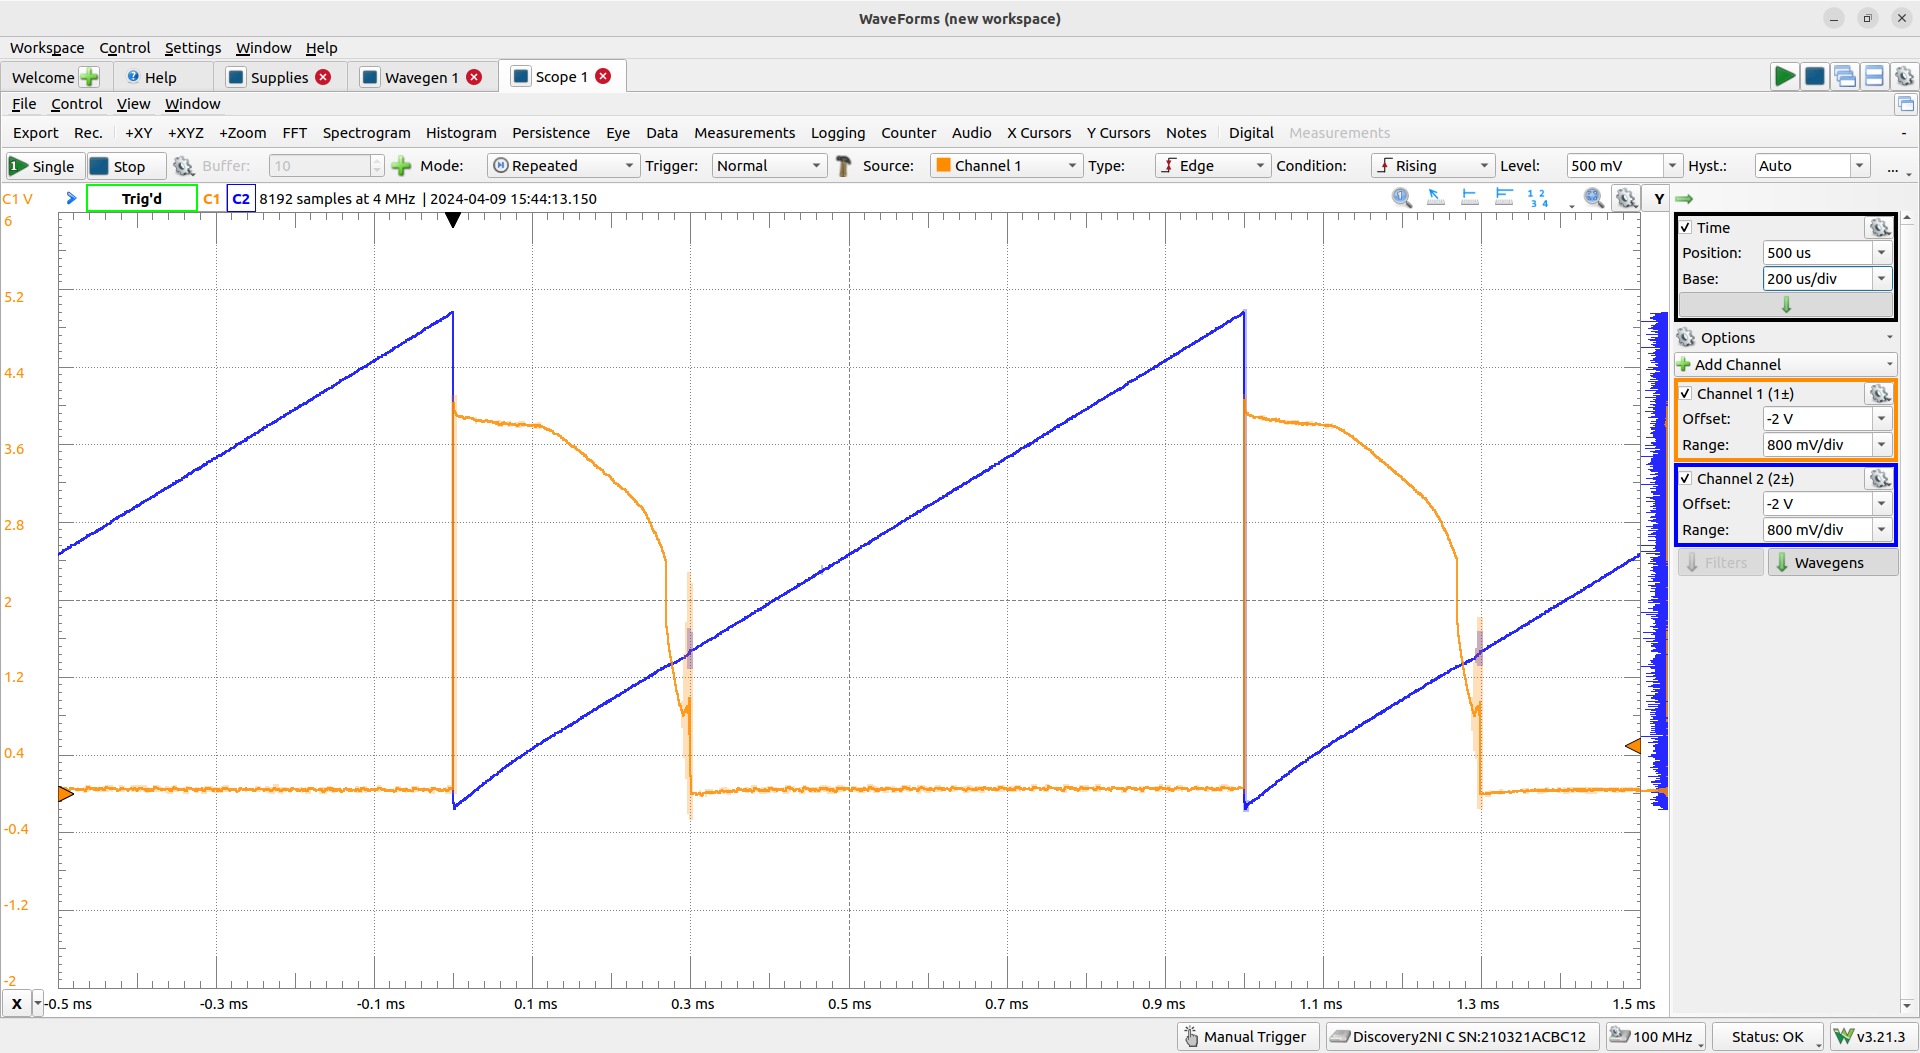
\includegraphics[scale=0.25]{fig1.png}
\caption{Segnale di rampa e di uscita NOT.}
\label{fig1}
\end{center}
\end{figure}

\begin{figure}[htp]
    \begin{center}
    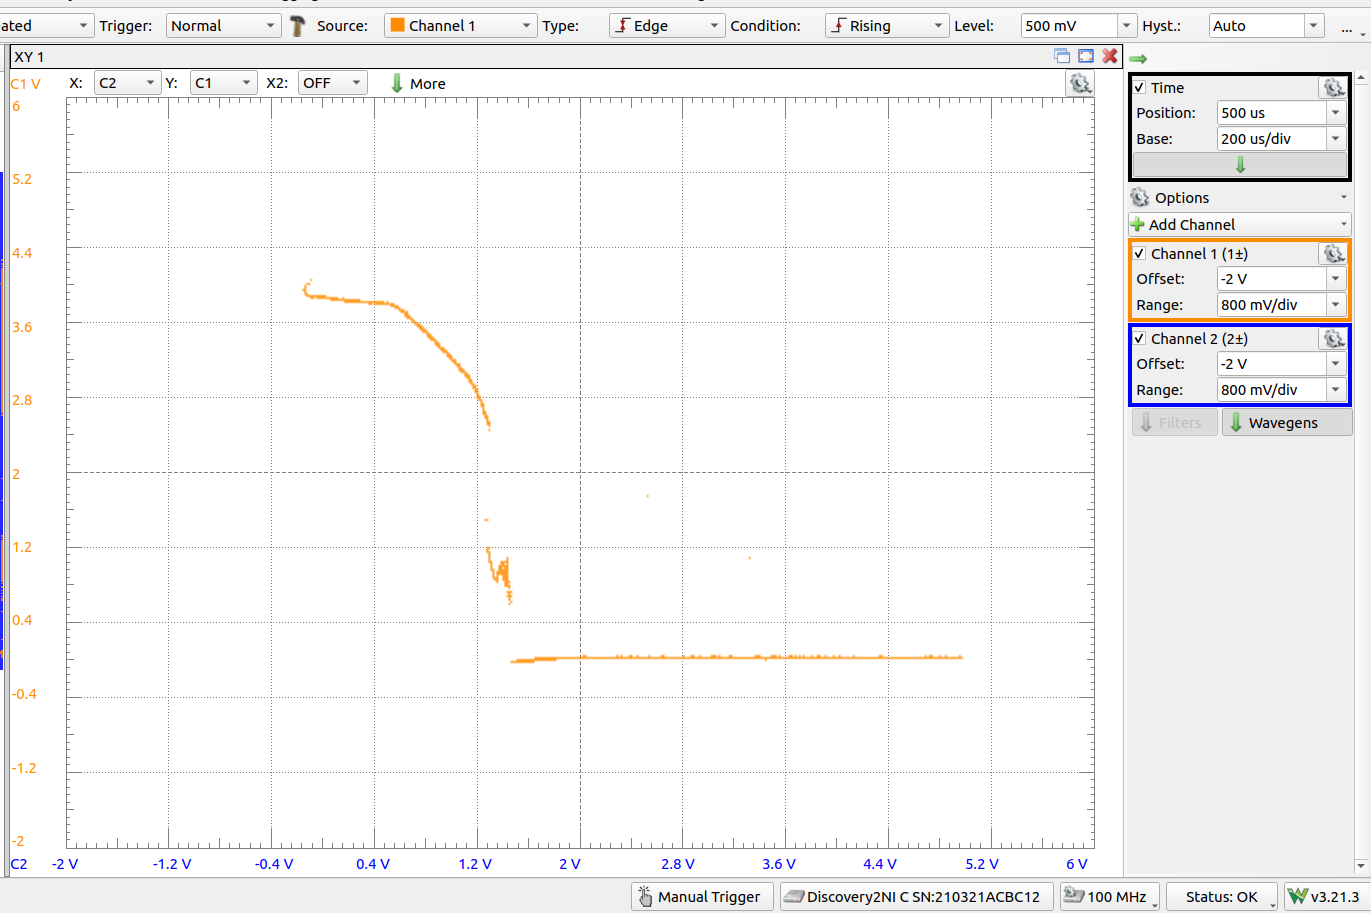
\includegraphics[scale=0.25]{fig2.png}
    \caption{Tensione in uscita in funzione della tensione in ingresso.}
    \label{fig2}
    \end{center}
\end{figure}

Le stime di $V_{OUT_H}$ (0.8 V in ingresso) e $V_{OUT_L}$ (2.0 V in ingresso) per ciascun membro del gruppo risultano rispettivamente 3.44 V, 3.49 V e 0 V per entrambi. I noise margin risultano quindi $NM_H = 1.44 V$, 1.49 V e il noise margin low è $NM_L = 0.8 V$. I valori ottenuti sono quindi molto simili a quelli riportati nel datasheet, infatti quelli del datasheet sono $NM_H = 1.4 V$ e $NM_L = 0.6 V$.

\subsection*{Misura del Fan-out della porta}
Inviando un segnale alto abbiamo misurato la corrente in ingresso $I_{IH} = (19 \pm 1) \mu A$. La corrente in uscita è invece $I_{OH} = (827 \pm 8) \mu A$. Il fanout risulta quindi $I_{OH}/I_{IH} = (43.5 \pm 2)$. IIL valore atteso per il fanout è 10, consistentemente con quello misurato.


Per stimare il tempo di risposta delle porte not si sono collegate in serie tutte le 6 disponibili, inviando alla prima di queste un segnale onda quadra, permettendoci di misurare all'ultima un tempo di risposta complessivo di circa $\delta t = 43 ns$. Dunque il tempo di risposta di una singola porta è di $\delta t_1 = 7 ns$, in accordo col valore di 8 ns del datasheet.

\begin{figure}[htp]
    \begin{center}
    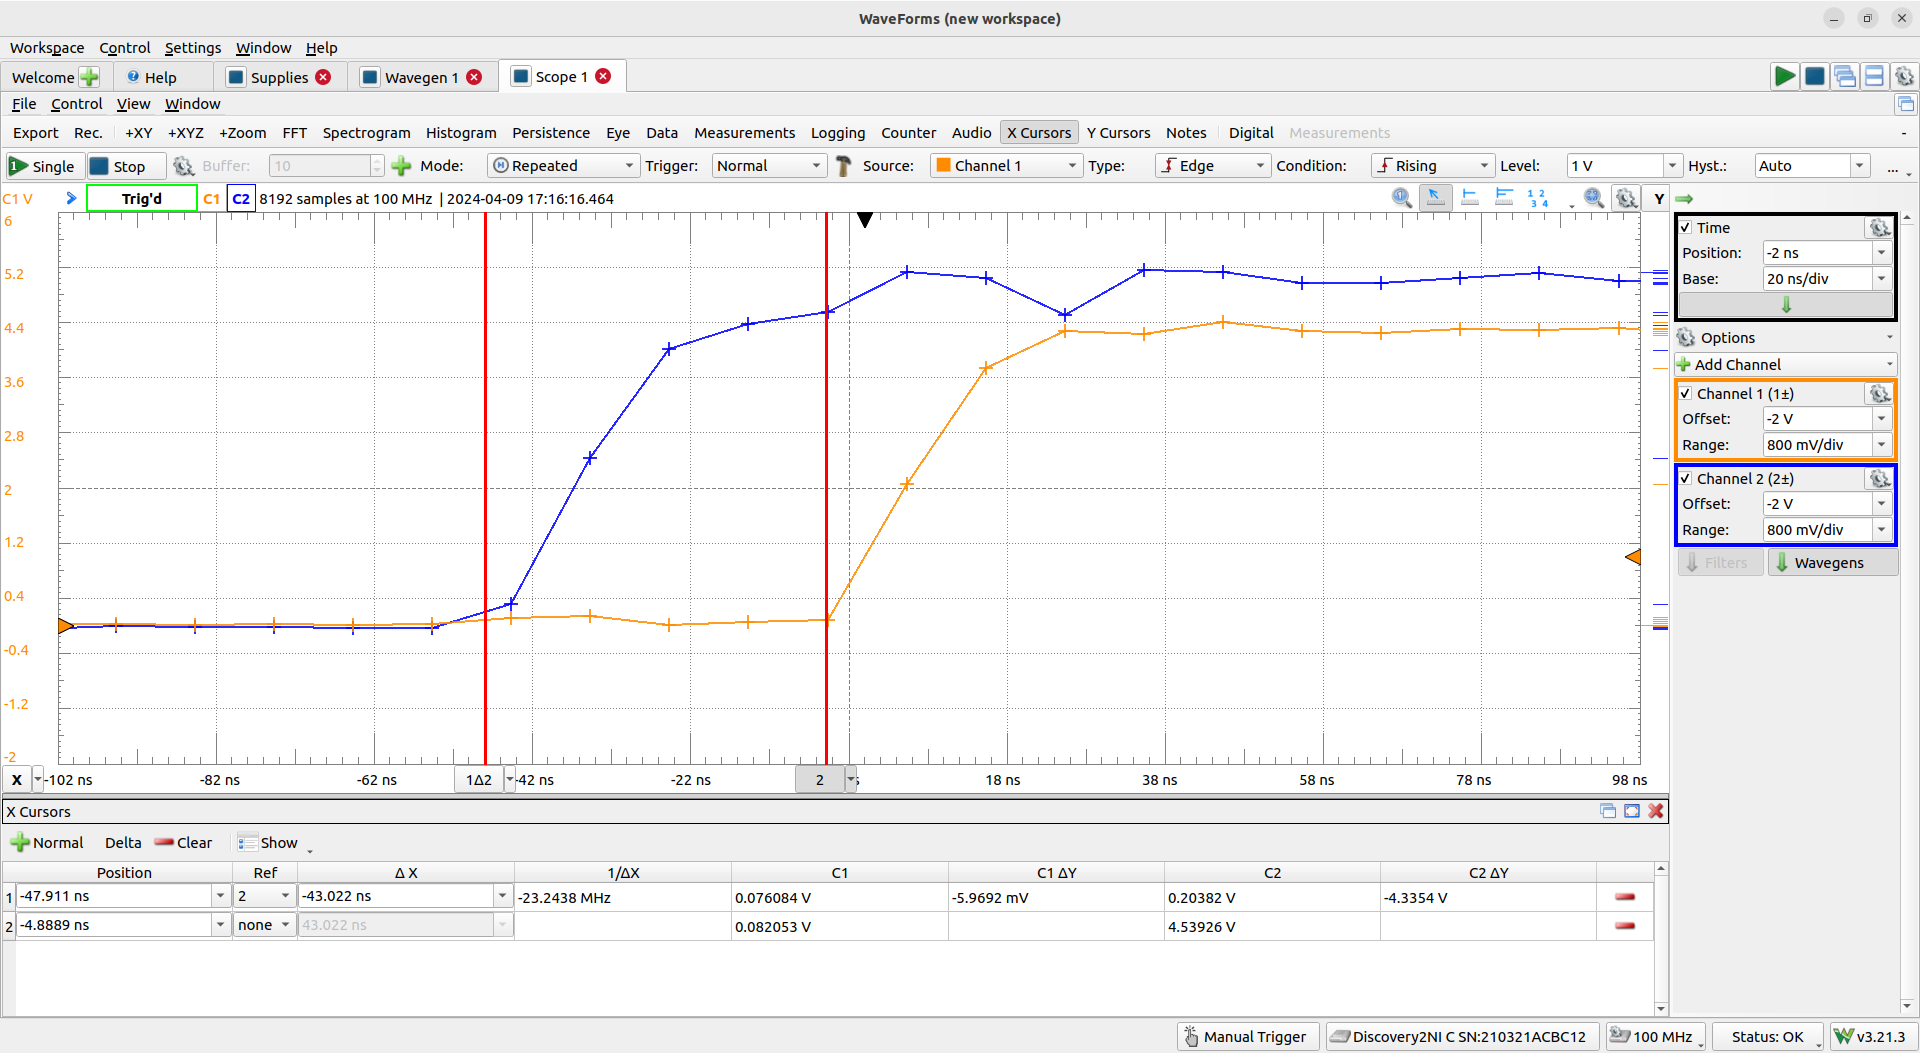
\includegraphics[scale=0.25]{fig3.png}
    \caption{Misura del tempo di risposta dell'integrato.}
    \label{fig3}
    \end{center}
\end{figure}

\section{Costruzione di circuiti logici elementari.}
\begin{figure}[htp]
    \begin{center}
    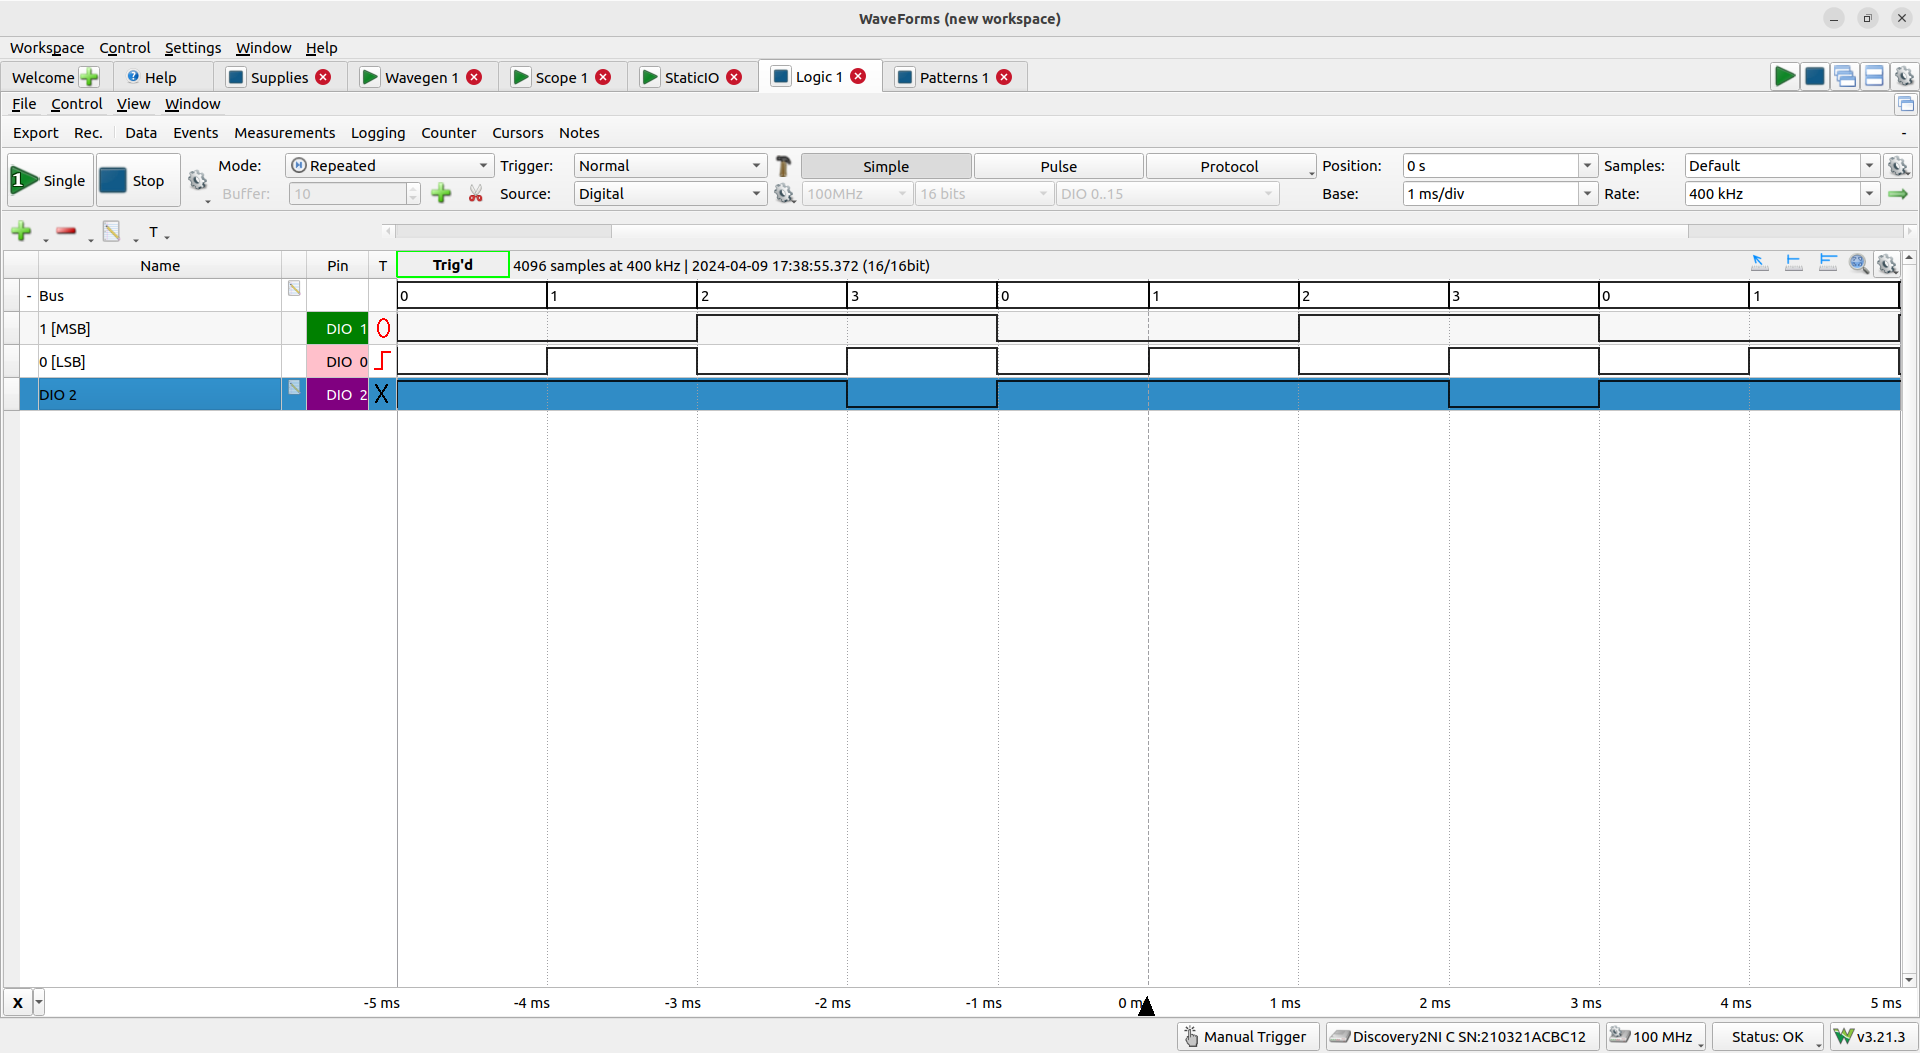
\includegraphics[scale=0.25]{fig4.png}
    \caption{Verifica della porta NAND (DIO 2 è l'output).}
    \label{fig4}
    \end{center}
\end{figure}

\begin{figure}[htp]
    \begin{center}
    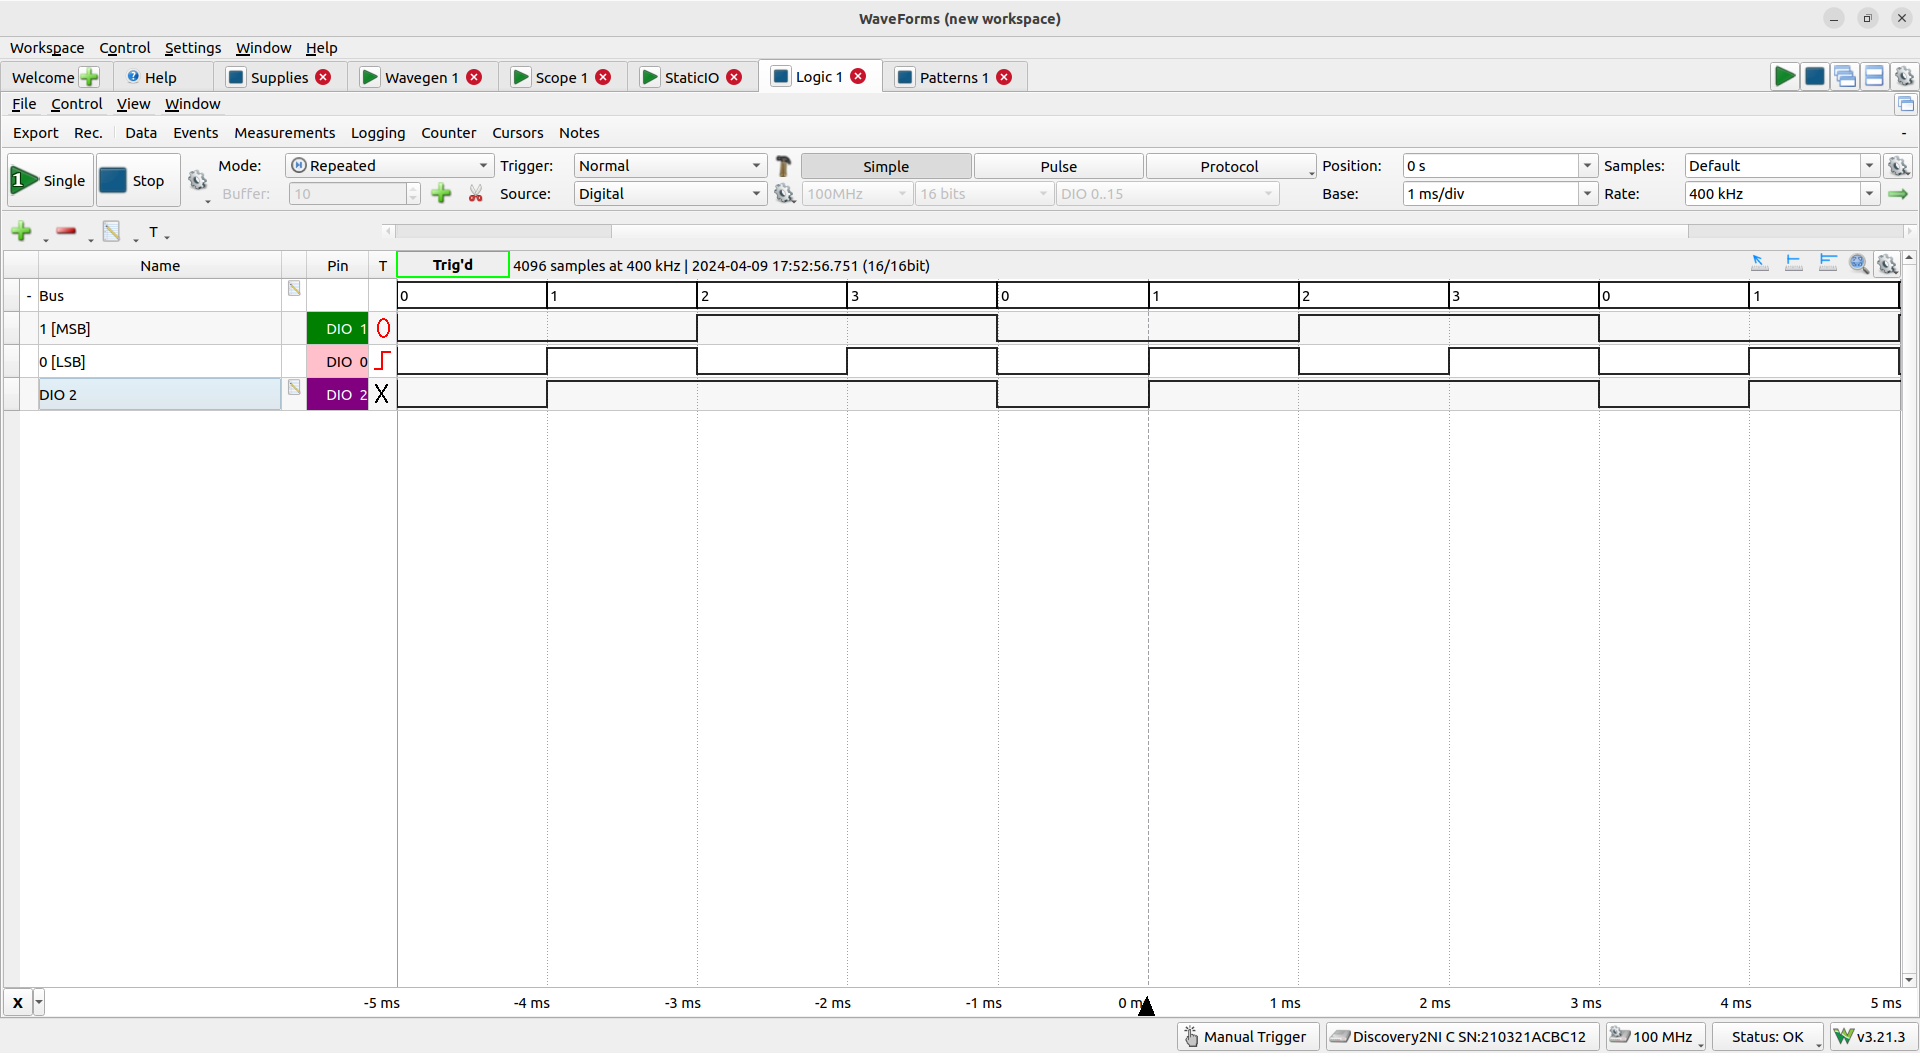
\includegraphics[scale=0.25]{fig5.png}
    \caption{Acquisizione della porta OR costruita con NAND come porta universale (DIO 2 è l'output).}
    \label{fig5}
    \end{center}
\end{figure}

\section*{Convertitore Gray-Binario}
Un convertitore Gray-binario a 4 bit da le seguenti codifiche per 5 valori arbitrari
\begin{align*}
    0000 \rightarrow 0000
\end{align*}
\begin{align*}
    0001 \rightarrow 0001
\end{align*}
\begin{align*}
    0011 \rightarrow 0010
\end{align*}
\begin{align*}
    0010 \rightarrow 0011
\end{align*}
\begin{align*}
    0110 \rightarrow 0100
\end{align*}

\begin{figure}[htp]
    \begin{center}
    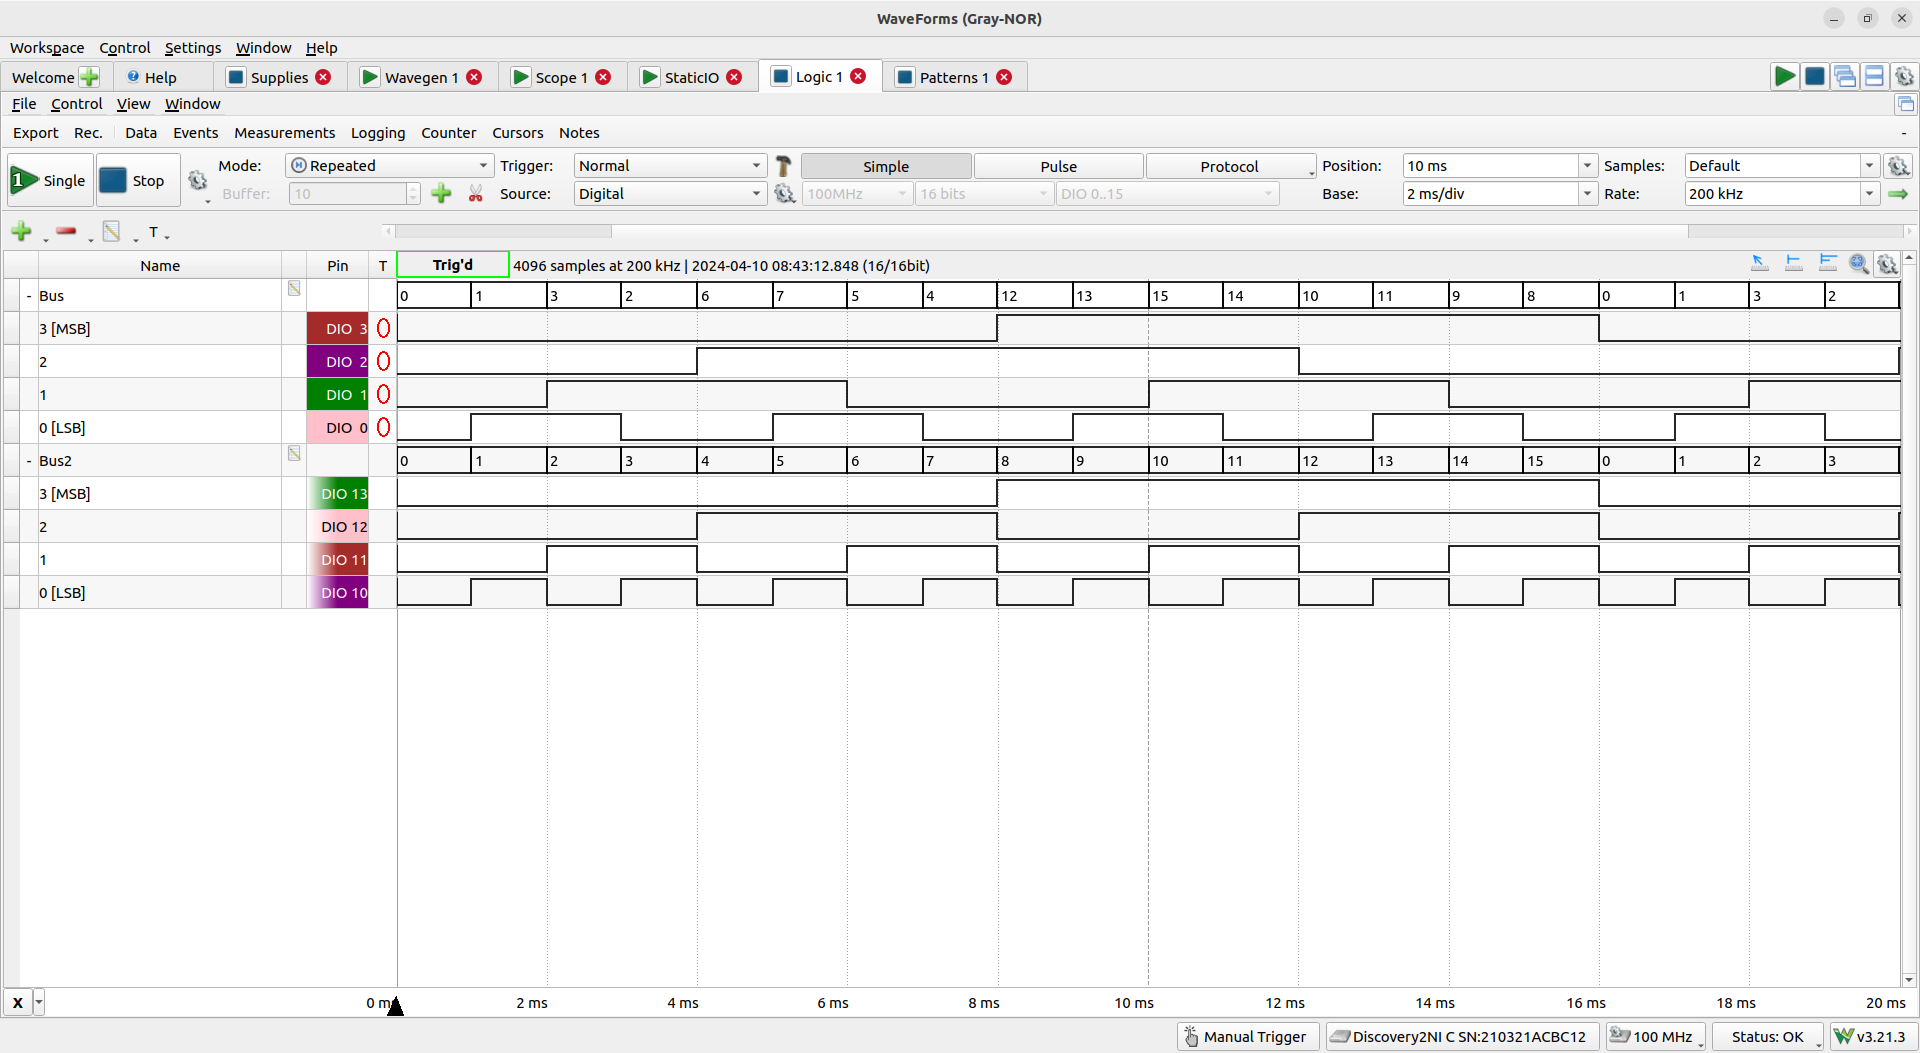
\includegraphics[scale=0.25]{fig6.png}
    \caption{Convertitore Gray-binario, DIO 0-1-2-3 in input e 10-11-12-13 in output.}
    \label{fig6}
    \end{center}
\end{figure}

\begin{figure}[htp]
    \begin{center}
    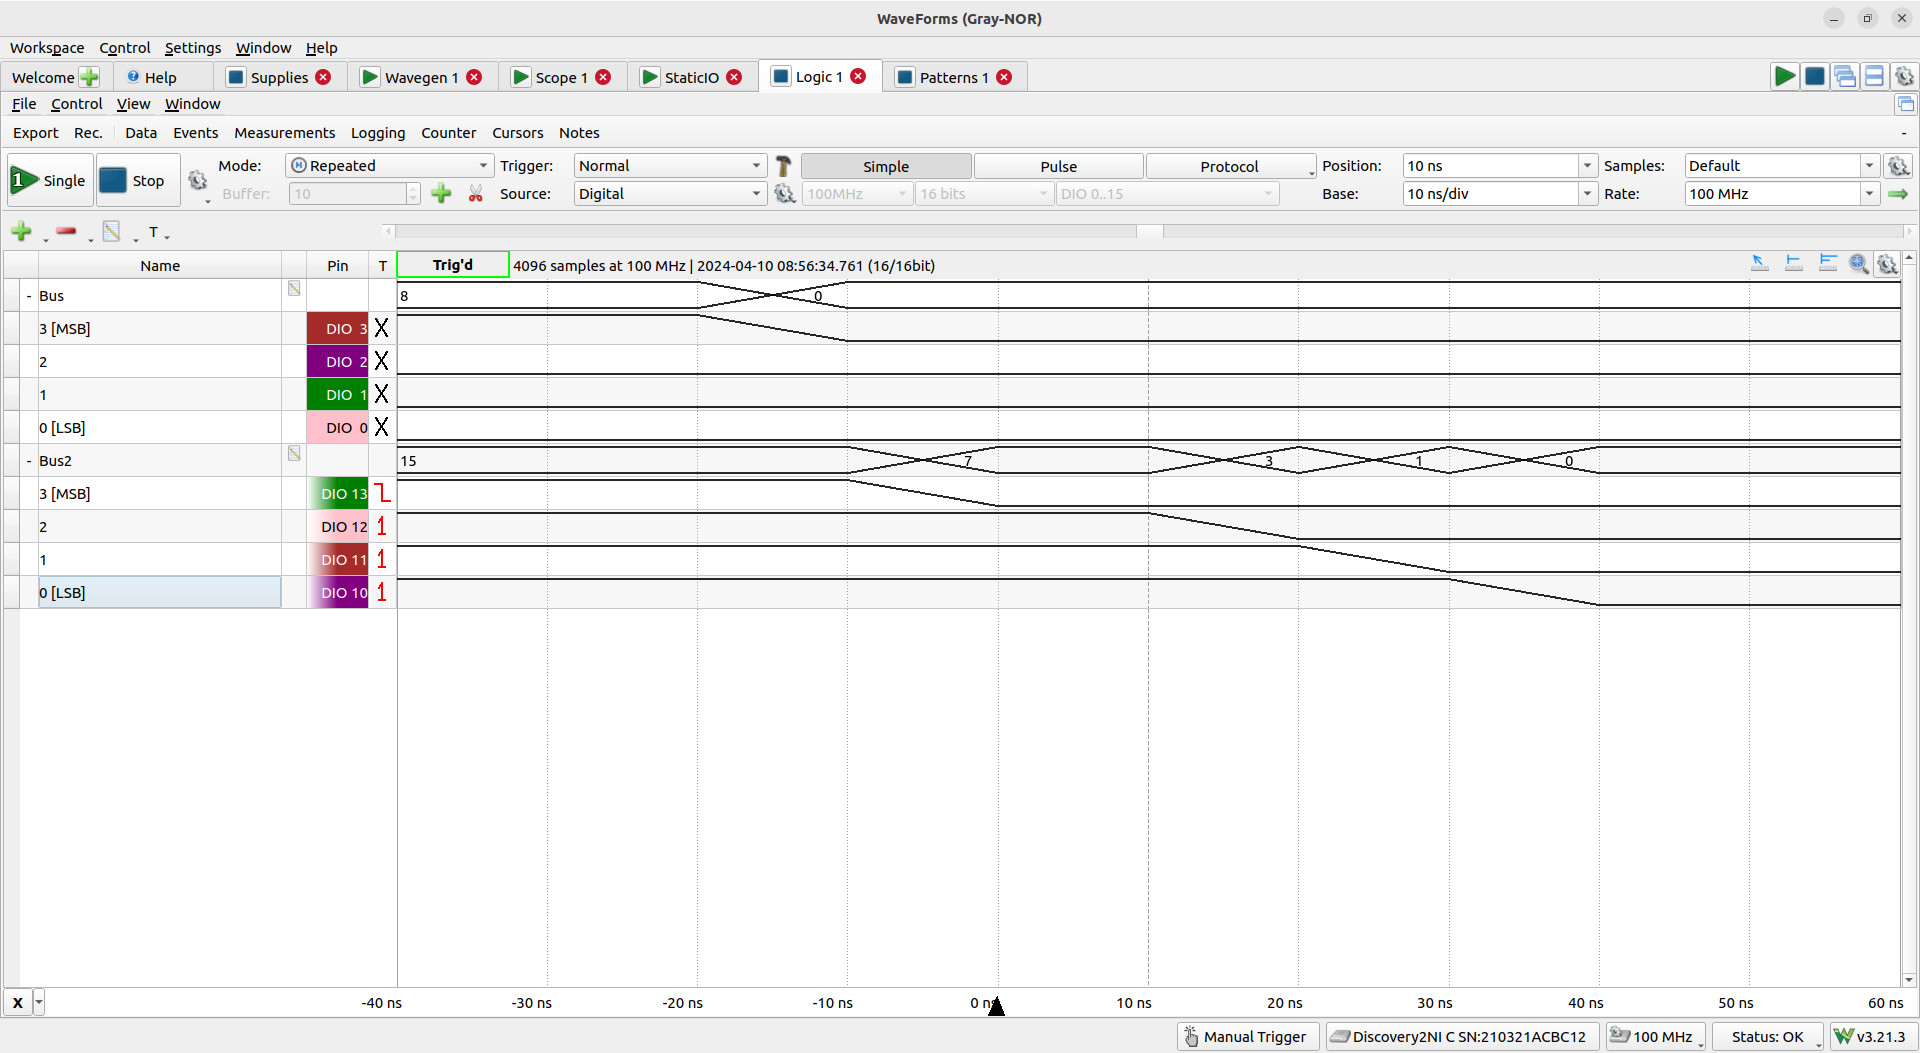
\includegraphics[scale=0.25]{fig7.png}
    \caption{Osservate della transizione in uscita dal numero 15
    al numero 0.}
    \label{fig7}
    \end{center}
\end{figure}

Nella transizione in uscita dal numero 15 al numero 0 si osserva quanto atteso: l'ultima porta di uscita (DIO 13) è la prima a effettuare il passaggio da segnale alto a basso, mentre le precedenti presentano un ritardo sempre maggiore. Questo ritardo è dovuto al fatto che uno degli ingressi di ciascuna porta XOR dell'integrato (che produce l'output $B_n$) coincide con l'uscita della porta che produce l'output $B_{n+1}$. Dunque è naturale che tra l'ouptut $n+1$ e $n$ ci sia un tempo pari al tempo di risposta della porta logica.

%da qui le indicazioni da seguire
\begin{comment}
    ​Laboratorio di Fisica 3 AVANZATO
    Prof. D. Nicolò, Prof. C. Roda
    ​ sercitazione N. D01
E
Caratteristiche porte logiche e semplici circuiti logici
L’esperienza di oggi ha molteplici scopi:
● Imparare ad utilizzare il Data-Sheet (DS) per gli integrati di porte logiche;
● Misurare le caratteristiche fisiche delle porte logiche e confrontare le misure con le
specifiche del DS;
● Imparare a progettare e costruire circuiti digitali combinatori applicando le regole della
logica booleana e le strategie di progettazione discusse a lezione.
ATTENZIONE: quando si dice “stimate” significa che si chiede una valutazione approssimativa
del parametro in osservazione senza quindi una valutazione dell’incertezza.
I circuiti integrati che verranno utilizzati sono di tipo Transistor Transistor Logic (TTL).
L’esperienza si articola su più parti:
a. misura delle caratteristiche statiche e dinamiche delle porte TTL, come esempio
utilizzeremo porte NOT contenute nell’integrato SN7404 (6 porte NOT);
b. costruzione di varie funzioni logiche fondamentali utilizzando esclusivamente porte
NAND (integrato SN74LS00);
c. utilizzo di chip che implementano funzioni logiche diverse per realizzare circuiti
combinatori complessi.
Cosa si deve consegnare:
● per la parte A stilare una relazione per spiegare come si sono fatte le misure ed illustrare i
vostri risultati. Per ogni gruppo si riportano i risultati di entrambe i membri NON come due
persone che non sanno nulla l’uno/a dell’altra/o ma come due persone che hanno discusso
come fare le misure e hanno trovato un accordo o, se non hanno trovato un accordo, sanno
motivare le differenti scelte.
● per le parti B fornire:
○ la derivazione analitica, utilizzando l’algebra di Boole, che trasformi la funzione
logica desiderata in soli NAND;
○ lo schema del circuito;
○ una acquisizione effettuata utilizzando le funzioni Pattern e Logic che dimostri la
funzionalità del circuito.
● per la parte C fornire una acquisizione che dimostri il funzionamento del circuito ed un
grafico temporale per motivare l’osservazione al punto 6.iii.
Parte A: Caratteristiche fisiche delle porte logiche
Familiarizzare con il data-sheet dell’integrato SN7404 (porte logiche
NOT), in particolare individuare:
● absolute maximum ratings;
● tensioni di soglia di ingresso VIH, VIL;
● tensioni tipiche di uscita VOH, VOL;
● correnti di ingresso e uscita IIH, IOH.
Se ci fossero dubbi sul significato delle variabili utilizzare il documento:
TI-UnderstandingDS.pdf che si trova nella Documentazione Tecnica sotto la cartella Integrati serie
74xx.In questa parte dell’esperienza non si vogliono fare misure con alta precisione ma verificare che la
porta sotto osservazione rientri o meno nelle specifiche del DS.
Collegare l’integrato sulla basetta in una zona centrale ed alimentarlo connettendo le tensioni 0V e
5V. Per semplicità di lettura degli schematici in questa scheda non sono mostrate le connessioni
dei pin di alimentazione dei vari integrati.
1) Tensioni di operazione. Connettere il canale 1 del Wavegen all’ingresso di una delle porte NOT.
Generare una rampa che vari tra tensioni 0-5V generando l’offset adeguato. Fate attenzione a
NON inviare tensioni negative in ingresso (anche se il diodo in ingresso protegge da questo
errore…).
a. Misurare la tensione VOUT in funzione di VIN e costruire il relativo grafico. Questa
operazione può essere fatta utilizzando la modalità XY dell’oscilloscopio oppure
salvando i dati su disco e analizzandoli con uno script.
2) Un modo per stimare il noise margin sulla nostra porta logica e` proposto qui sotto (vedi figure):
a. stimate Vout per VILMAX (Vout-H);
stimate Vout per VIHMIN (Vout-L);
valutate il noise margin high (NMH) come Vout-H - VIHMIN;
valutate il noise margin low (NML) come VILMAX - Vout-L;
Nota: la stima del noise margin eseguita secondo questa procedura è conservativa in
quanto VIHMIN e VILMAX sono presi dal datasheet. Il circuito integrato sotto test
potrebbe avere valori migliori, per esempio potrebbe riconoscere come Low anche
valori superiori a VILMAX.
b. Ottenete i Noise Margin dal data-sheet e confrontate i valori ottenuti al punto
precedente per valutare se la porta sotto osservazione rientra nelle specifiche.
Figura 1: definizione dei simboli per la stima del Noise margin in una porta NOT.
2) Misura del Fan-out della porta (misurazione statica) – si vuole misurare il valore del
fan-out della porta per un valore logico alto. Per simulare il carico delle porte si utilizza un
potenziometro da 10 kΩ. Per fare questo seguire i seguenti passi:
a. Misurare la corrente in ingresso IIH inserendo l’amperometro in serie all’ingresso della
porta. IIH è la corrente (I) in ingresso (I) quando un valore di tensione alto (H) è
applicato a quel input.
b. Misurare la corrente in uscita IOH utilizzando in serie all’uscita della porta un
amperometro a sua volta in serie a un potenziometro da 10 kΩ. IOH è la corrente (I) in
uscita (O) quando i valori in ingresso sono tali da generare per quell’uscita un valore di
tensione alto (H). Applicare all’ingresso una tensione tipica per lo stato L (0.2 V). Per
misurare IOH variare la posizione del potenziometro fino a far scendere a circa 3.4 V ilvalore di VOUT (valore indicato come VOH tipico per la porta). Misurare quindi il
valore di IOH in queste condizioni.
c. Valutare il valore del fan-out della porta con le vostre misure.
d. Valutare il valore del fan-out dalle specifiche del DS e dire se la porta sotto
osservazione rientra nelle specifiche.
3) Tempo di propagazione
Si vuole stimare il tempo di propagazione delle porta NOT che e` dell’ordine di una decina di
nanosecondi. Per ovviare alla non sufficiente risoluzione temporale del nostro AD2
colleghiamo le 6 porte NOT in serie in modo da misurare il tempo di propagazione delle 6
porte NOT infatti.
Generate il segnale con wavegen (attenti a inviare segnali tra 0 e 5V) ed utilizzate
l’oscilloscopio (non Logic … perché ?) per misurare il tempo di risposta delle 6 porte. Stimate
il tempo di risposta medio della singola porta e dite se la vostra stima rientra nelle specifiche
riportate su DS.
Parte B: Costruzione di circuiti logici elementari.
Rimuovete il chip SN7404 dalla basetta. Identificate due integrati tipo
SN74LS00 contenenti ciascuno 4 porte NAND a due ingressi. Riferitevi al
data-sheet dell’integrato per tutti i dettagli.
4) Tabella di verità porta NAND
a. Osservate la tabella di verità della porta NAND utilizzando la funzione StaticIO di
WaveForms, in particolare verificarne la tabella di verità (statica) posizionando gli
interruttori nelle quattro possibili posizioni.
b. Utilizzando le funzioni Pattern di Waveform producete le quattro possibili coppie di
valori in ingresso e con la funzione Logic acquisite questi due segnali assieme al
segnale in uscita e riportate il grafico nella relazione.
5) Circuiti con porte NAND
Progettare, costruire, e verificare la tabella di verità per i seguenti circuiti utilizzando solo porte
NAND. Cercate di minimizzare il numero di porte utilizzate.
Consiglio: state attenti a riutilizzare i circuiti che possono essere utili in più punti.
i. circuito OR (2 ingressi – 1 uscita)
ii. circuito che permetta di assegnare all’uscita il valore di uno dei due ingressi a singolo
bit tramite il valore di un terzo ingresso (3 ingressi – 1 uscita).
iii. circuito XOR (2 ingressi – 1 uscita)
Per ognuno di questi fornite:
● la derivazione analitica, utilizzando l’algebra di Boole, che trasformi la funzione
logica desiderata in soli NAND;
● lo schema del circuito;
● una acquisizione effettuata utilizzando le funzioni Pattern e Logic che dimostri la
funzionalità del circuito (come al punto 4.b).
Parte C: Costruzione di circuiti logici complessi.
Rimuovete i circuiti precedenti dalla basetta.Identificate il chip SN74LS86 contenente 4 porte
XOR.
6) Convertitore Gray-BinarioIl circuito in figura provvede a convertire un valore a 4 bit dalla codifica Gray in Binario
utilizzando un unico integrato SN74LS86.
a. Verificate che il
disegno del circuito sia corretto calcolando il valore in uscita dal circuito per almeno 4
valori diversi in ingresso
b. Per il convertitore Gray → Binario:
i. verificate il funzionamento del circuito utilizzando Pattern per generare un
contatore a 4 bit con la codifica opportuna e osservando l’uscita con Logic
(come ai punti precedenti);
ii. osservate su una scala molto stretta (30ns) la transizione in uscita dal numero 15
al numero 0;
iii. motivate l’osservazione del punto precedente tenendo conto del tempo di
propagazione necessario;
iv. riportate tutti i grafici necessari a dimostrare il funzionamento del circuito.
Schematici su SystemVision:
● Convertitore Binario-Gray https://www.systemvision.com/node/415646
● Convertitore Gray-Binario https://www.systemvision.com/node/415619
7) Sommatore - Facoltativo
Andremo a realizzare un circuito sommatore di due
numeri A e B a due bit. Per fare ciò si utilizzerà un
circuito Half-Adder per i primi due bit (semplificando
rispetto all’utilizzo di un FA visto che il primo carry-in
nullo) e un Full-Adder per combinare il carry del
primo stadio con i due bit più significativi dei valori in
ingresso.
èa. Per la realizzazione del circuito sono necessari:
i. 1 chip SN74LS08 (Quad AND)
ii. 1 chip SN74LS32 (Quad OR)
iii. 1 chip SN74LS86 (Quad XOR)
b. Identificate nel circuito i due segmenti Half-Adder e Full-Adder, costruiteli
indipendentemente utilizzando lo schema visto a lezione e verificatene qualitativamente
il funzionamento.
c. Connettete il bit di carry dell’output dell’Half-Adder all’ingresso del Full-Adder.
Producete una prova del funzionamento come sommatore utilizzando Pattern e Logic
(come ai punti precedenti).
d. Aggiungete alla basetta 4 LED verdi e un LED rosso con le opportune resistenze di
limitazione.
Utilizzando la funzione “ROM” di Pattern create una tabella di verità che utilizzi come
input l’output del sommatore (incluso il carry) e che controlli i LED per formare un
indicatore “a barra” :
i. se il carry è H, accendere solo il LED rosso, si è avuto overflow nella somma;
ii. se il carry è L, accendere un numero di LED verdi proporzionale al valore della
somma (se il valore in ingresso è 0 nessun LED acceso, un led acceso se il
valore della somma è 1 e così via…).
Fornite nella relazione la tabella di verità utilizzata per la ROM (potete utilizzare il
simbolo ‘X’ per indicare i valori “do not care”) e tutto il materiale necessario a
documentare il vostro lavoro e dimostrare il funzionamento del circuito.
\end{comment}

\end{document}


